% Chapter 3

\chapter{Research Methodology} % Main chapter title

\label{Chapter3} % For referencing the chapter elsewhere, use \ref{Chapter1} 

\lhead{Chapter 3. \emph{Research Methodology}} % This is for the header on each page - perhaps a shortened title

%----------------------------------------------------------------------------------------

\section{Introduction}

The proposed information visualisation model is discussed and substantiated through design flow charts. In the first part of the chapter, a brief introduction to existing information visualisation model along with the proposed model is highlighted. The research model presented in this chapter is further explained with extracted code sample from the application developed for proposed visualisation model in the next chapter. The proposed visualisation model is validated through three experiments. The next two chapters are based on different experiments while further experimentation and comparative analysis discussed in chapter 7.

\section{Seven Stages of Data Visualisation}

The process of understanding data begins with a set of numbers and a goal of answering a question about the data. The steps along this path can be described as follows \cite{fry}:

\begin{enumerate}
\item Acquire - obtaining data from local, remote sources through web services or direct data set access.
\item Parse - organising and giving structure to collected data in the system environment. 
\item Filter - removing all but the data of interest.
\item Mine - the application of methods from statistics or data mining, as a way to discern patterns or place the data in mathematical context.
\item Represent - determination of a simple representation, whether the data takes one of many shapes such as a bar graph, list, or tree graphs.
\item Refine - improvements to the basic representation to make it clearer and more visually engaging.
\item Interact - the addition of methods for manipulating the data or controlling what features are visible.
\end{enumerate}

\begin{figure}[H]
\centering
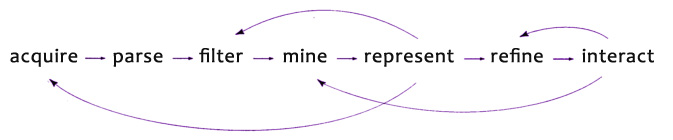
\includegraphics[scale=0.6]{chapter3/J_Fry_V}
\caption{Fry's Visualisation Model \cite{fry}.}
\end{figure} 

The research model shown in Figure 3.1 will be adapted for data visualisation which is a complete data visualisation process but the focus will remain on important elements of visualisation process and adjustment to process and development of the model to meet the requirements of small to medium size businesses and individuals with easy to use system approach. The research model is explained in the following section.

\section{Proposed 4 Stages of Visualisation}

The proposed 4 stages of information visualisation model is a complete set of action which could be applied to any kind of data set for data analysis and exploration purposes as presented in Figure 3.2.  

\begin{figure}[H]
\centering
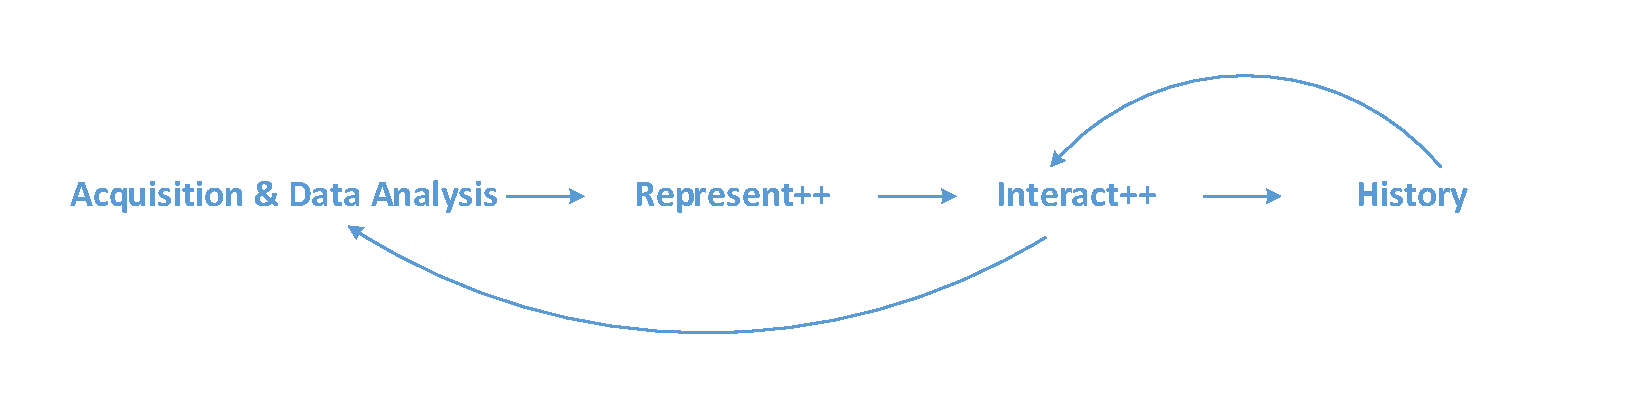
\includegraphics[scale=0.59]{chapter3/model}
\caption{Proposed Visualisation Model}
\end{figure} 

The first step of the information visualisation model proposed in this research is acquisition and data analysis. This part explains how complex raw data sets are converted into a normalised and easily retrievable data structure which is then passed onto the data representation layer. The data representation layer processes retrieved data from the database into visualised forms requested by the user or requests initiated by the predefined instructions by web intelligent agents. The data representation or represent++ layer pushes processed visualised data on to the interact++ layer where user and the computer system or application interaction take place with the end user. The users at the interact++ layer could request further analysis of the data and thus instructions are sent to the acquisition and data analysis layer to re-process information for more insights about data processed in any given data set. The acquisition and analysis model re-sends requested information to data representation and exposed to users at the interact++ layer. History layer where stored or exported reports are processed. The information could be requested by the users at the interact++ layer and made available upon demand. This layer is very important as re-using system generated particulars in the past and thus making this layer extremely important for version history control or comparison purposes.\\

Transactions tagging and linked data visualisation along with multi-coordinate and multi-attribute visualisation techniques and approaches were absent in the existing tools and models. Similarly, robust and effective solutions to export and store visualised content was not available in the existing tools. Acquiring and processing complex and diverse data elements. Visualising complex data elements into simplest of forms, thus making it very easy for the users to analyse data more effectively without any prior knowledge of the visualised content. The concept of this research revolves around information visualisation through mashup application for enterprise practice to understand huge transactional data for resource and decision making purposes, focus is on understanding data through visualisation, interactivity of the system with end user, storage of generated results for re-use and comparisons purposes and finally light weight mashup applications - resource friendly and economical. All the four stages of the visualisation proposed in the visualisation model above are further explained in more detail below.

\subsection{Acquisition and Data Analysis}

Data is a term, that's thrown around a lot in modern business circles. The problem is, it's such a wide term that it can sometimes be difficult to define. To clarify - data can be any kind of fact, figure or textually based data that can be analysed and processed using computers \cite{chamberlin1976sequel}. Because of the recent surge in data analysis, the processing power and storage capacity of modern computers has been hugely affected - and this has played a vital role in further data growth. There are many types of data stored in computers and vaults today. For example, transactional data, as the name suggests, this refers to data acquired during transactions. This can include sales, purchase or even cost and accounting data, and this often relates to the business operations side of things \cite{abadi2009data}. Some could be categorised into non-transactional data type, this data is found outside of direct business statistics - and is instead more about industry forecasts and economic data \cite{herlihy1993transactional}. Finally, meta data is how it is defined and what class of data each segment belongs in, and contains information on the data, including how it is structured and defined and where it came from \cite{harris2009research}.
\end{itemize}

Data analysis plays an important part in understanding complex data. By going through the computational data analysis and representation process, chunks of data that were meaningless can now be presented in an easy to understand and clear way. The different approaches to understanding data and how it is typically retrieved from various data sources for analysis will be discussed. The most important factor in data analysis is that it leads to information. This information is essential to understanding business and identifying patterns, allowing us to hone business models to work at their highest efficiency. To combine the understanding of data with the analysis of patterns, associations or other relationships, and the information is a very powerful tool. It will be useful to understand, for example, how many sales a single staff member converts in one month, which can help in streamlining the performance of the sales team. Data harvested by the system on a certain staff member can be analysed, and can produce a figure, giving an answer to the question raised regarding business sales \cite{hair2006multivariate}. The information gained can then be used to discover new patterns and trends - letting users to explore possibilities and predict outcomes before taking the risks. For example - users can use data analysis and information to find out how good a certain staff member is at converting sales, which of the sales force has the lowest conversion rate and who has the highest, and all of this can lead to a greater understanding of sales force, with facts and figures to  evidence it \cite{larose2014discovering}. Most of the data that will be processed in this research using modern computational data processing and analysis techniques which has been harvested in a readable format. Disks are one of the most common ways to store large or small volumes of data, and is easy to source and interpret. Data is simply removed from the disk and processed by data analysis web intelligence agents, with little computer involvement at this stage. This is because the data stored on disks is already in a human readable presentation format such as PDFs or JPEGs, and is easy to decipher and interpret without added help.  

A more modern addition to the acquisition of data is from network streams  - a technique made possible by the Web 2.0 era. One of the most common examples of data acquisition from networks is usually through network streaming - particularly data feeds generated by rich data sources. This can be anything from a news feed generated by a news website to a product and transaction feed from a retailer. However the downside lies in the huge variability in network streaming - there is no consistent format for the data, and it can vary not only from source to source, but within the same source. Luckily there are some commonly used themes that makes it easier for the data acquisition agents to retrieve the information required from such sources in a way to understand and interpret \cite{nandy2014real}. A database is a much easier source to collect data from, simply because a database by nature is a collection of data in organised and formatted structure. Because the data is so structural it can be easily retrieved and analysed when required \cite{urban2014integrated}. The majority of databases are made up of tables, and require a set of connections to enable data streaming - and these can be made using database drivers. As an example, a table within a database could be titled student. This table will hold all of the student data - including name, address, phone numbers etc. This data would lie dormant until it is retrieved via a query. Queries are usually a command or instruction made in SQL (Structured Query Language) and issued to the database. An example would be:

\begin{listing}
SELECT student_name from student WHERE name is smith;
\end{listing}

This query would produce rows of data that match the search criteria (i.e. where the students name is smith). While the above is a very basic query, it is the general way in which the information is retrieved from databases - by sending instructions to the required data. For large databases with a huge volume of data, more complex queries can be manipulated to gather the right data. The only major drawback in acquiring and processing information from databases is the retrieval process. Databases work on an information pull and push concepts (where information is only dispensed when a command is issued of a certain event occurs), and this limits the amount of data one can access in a effectively. As the data is only retrieved when specific queries are issued, it is not always available for large volume processing and analysis, and one must follow this push and pull structure for every element, and every different type of information required.

The acquisition of data has itself become a vital part of the information processing practice, and systems are being developed that will know the relevant attributes needed and make it available for processing. For example, if the system only needed to know the name and address of a student, it could ignore all other fields as are not required for that particular search. The data acquisition can vary depending on data source and methodology, our computational data analysis and representation model can acquire the majority of data from both relational databases and different data feeds in order to validate the visualisation model. Data parsing is the technical term for splitting a large data set into much smaller sections through defining criteria before structuring and organising it. This process makes it much easier for automated systems to interpret, manage and transmit the data. Any data could be acquired through the parsing method which can then be structured and organised in multiple ways to allow data to fit into a certain system environment. Data sets usually consist of various large data elements, it's not always feasible to process all of it. Often there will be elements of the data sets that are not required or completely irrelevant to the analysis being done. The proposed system only allows the relevant sub-sets of data to be retrieved, and those that don't meet the conditions or criteria are not harvested in the first place. For example, instead of retrieving all the rows of data from the student table, the user or even the system can set parameters and condition criteria to help filter down the elements required before fetching  from the system. The filtering is the process of removing unwanted or un-usable information from the data sets. Closely related to user input, the systems will refine the data sets when requested , to ignore information that does not fall within the specifications, or that is irrelevant or repetitive. While some data is removed from the data sets before these are processed for representation - it can only be done if there is user defined conditions put in place by web intelligence agents in the pre-defined data filtering stage. Data filtering could have a secondary use. It can be used to restrict access to sensitive information within databases - allowing parameters to be set that restrict user access to certain information such as credit card numbers, social security numbers and in some cases personal information. This makes data filtering the perfect solution for managers and directors who are wanting to hide such sensitive data, and avoid an ordinary staff member stumbling across it.
 
Larger data sets can sometimes prove challenging to analyse, but often mined for a number of different things - such as a deeper understanding of data categorisation which can help improve the analysis. There are many different kinds of categorisation, but may have different names tend to be for the same purpose, and can be summarised as follows:

\begin{itemize}
\item Grouping Data: Data can be grouped together to help explore patterns and analyse the data sets in more detail. How many bookings staff convert in a single day? Finding the two aspects of date and conversion rate and combining it will provide the answer. Data is stored or extracted into a more logical pattern to further explore the data relationships. For example - what percentage of conversion does a staff member of a particular organisation do in a single month. To answer this question, one need to examine how much that staff member contributes to all the sales in the company, and explore in detail the relationship between sales transaction and each staff members conversion rate \cite{hedges2014statistical}.

\item Data Relationships: This refers to exploring the relationship between various data elements to allow us to find any association or relationship. This could be used to find out why the conversion rate falls when a staff member reaches their target \cite{vidulin2014combining}.

\item Data Patterns: Data can be mined to explore different patterns of behaviour within data. This could be used to discover why the conversion rate is always at its highest when staff members haven't reached their targets \cite{singh2013web}.

There are many elements of data mining that relate and mix with each other, there are a few data mining principles that always hold true:
\begin{itemize}
\item Scraping or extracting information from a data set onto a particular segment
\item Stocking and maintaining information in multidimensional data sets
\item Connecting analytic systems and data sets
\item Making data available in a useful form
\end{itemize}
\end{itemize}

It should be fairly clear that data analysis is all about collecting statistical data and analysing it to predict behaviours, identify trends and explore new insights into the business. There are many techniques for data analysis, such as Single Variant (where data is analysed for a single-variable distribution) and multiple Variant (where it is analysed for multiple dimension attributes) Data Analysis, and all of these techniques can be practiced. But the main message is that the researcher using the techniques should be fully focused on the approach adopted, and be completely satisfied with the analysis process. Data visualisation is a multiple layered practice, but at the heart of it all is the structuring of data. In the proposed methodology the system will establish whether the information visualisation request that is initiated from an Enterprise 2.0 or a non-Enterprise environment. 

In an Enterprise 2.0 environment, the proposed system will already be aware of the environment and will have pre-authorised direct access to the data sets through web services and API's (Application Program Interface) or web intelligent agents. Various mashup applications will also be able to understand and interpret the data structure, also directly access and pull the relevant information for visualisation purposes. Because of this, this versatile system will already have multiple connections and entry points for the data sources in real time - and if the source should change in any way then the proposed system application will be automatically updated with data acquired from the source. The processing in a known environment (Enterprise 2.0) will facilitate the first four steps (acquire, parse, filter and mine) through API's and web services or through web intelligent agents(PHP predefined functions). For example, if the application now requires sales figures, various mashup systems and web intelligent agents could log in and access the sales figures parameter through API's. This data would be drawn out in XML format or SQL Queries and be passed straight to the represent layer for visualisation.

If the environment is an unknown (a non-Enterprise environment) then this can make accessing data sets through API's extremely difficult as the application or the source might or might not be able to support web services or remote data retrieval. This can also mean that the data is stored in an unknown structure. In these cases, the mashup application can request data through a custom tool called visualixer, this tool has been specially created and developed for the non-enterprise data sets. The tool has the ability to read, mine, filter and parse data acquired from the importer tool and has a specialised data representation layer which visualise data and push it to the user at the interact++ layer. The visaulixer and its features are discussed in more detail in chapter 6.

\begin{figure}[H]
\centering
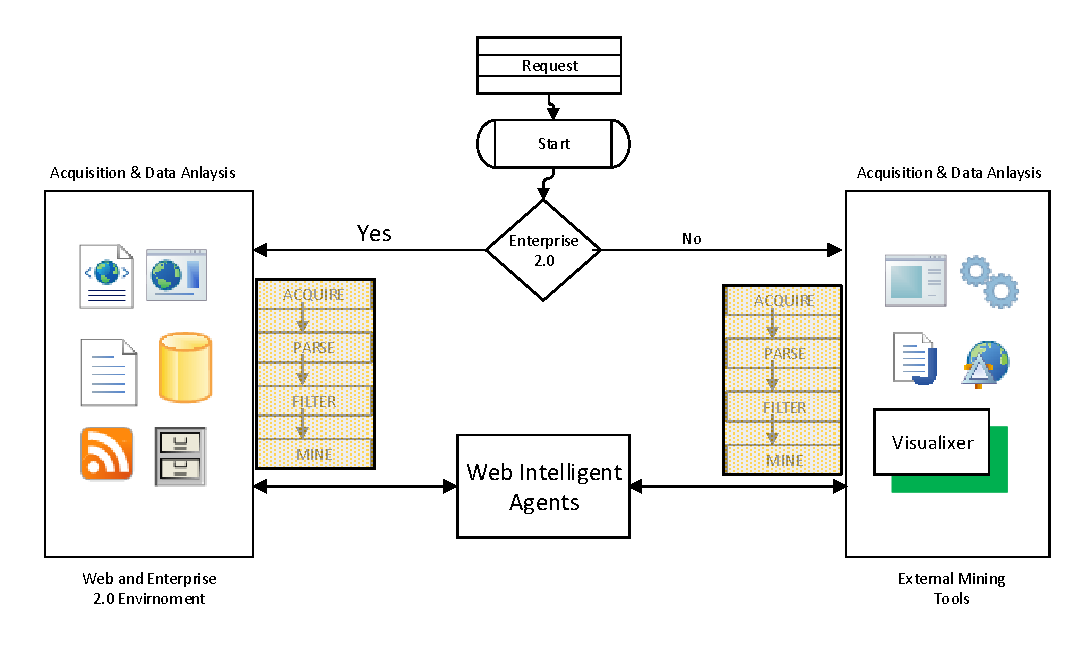
\includegraphics[scale=0.8]{chapter3/data_analysis_flow}
\caption{Data Analysis System Flow Chart}
\end{figure} 

Figure 3.3 shows the data analysis flow in the system. In Enterprise 2.0 environment where data is in a normalised or known state, information is then retrieved through web intelligent agents(PHP functions). However, if the data is not in enterprise or normalised format it is then passed onto a more detailed data analysis process for which a bespoke application is developed called visualixer which is further explained in chapter 6. 


\begin{figure}[H]
\centering
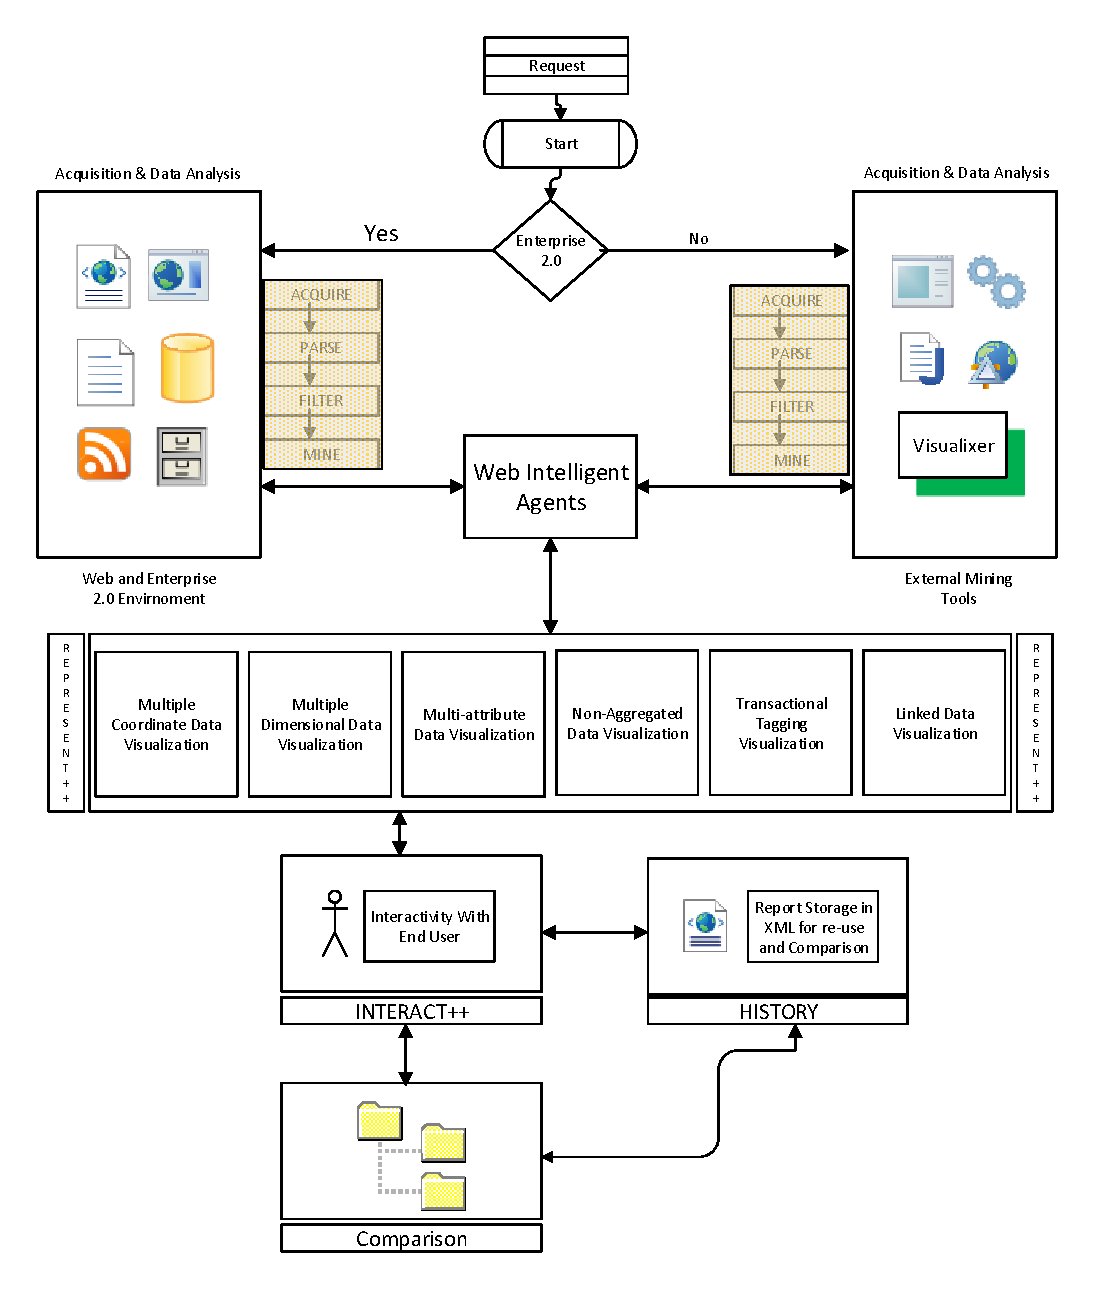
\includegraphics[scale=0.8]{chapter3/system_flow_chart_full}
\caption{Proposed Theoretical Visualisation System Flow}
\end{figure} 

The full system flow chart is presented in Figure 3.4, in the next section represent++ where data representation process is further explained in more detail below.

\subsection{Represent++}

This layer is called represent++ and it is responsible for visualising data and producing visualised content. The layer is labelled represent++ because it is different from Fry's represent layer \cite{fry}. The represent++ layer will remain mostly the same for different type of data processing and visualisation, regardless of whether the data came from an Enterprise 2.0 or non-Enterprise environment. This is incredibly useful as it has become a key step in the understanding of transactional data and non-transactional data. This layer has been contributed with new approach in processing and visualising data as this layer has been extended into more elements, for example multi-coordinate visualisation, non-aggregated data visualisation, transactional tagging visualisation and linked data visualisation.

Multi-coordinate visualisation is used at the representation layer, which allows users to put visualised data into coordinated views for ease of understanding. If one element of the visualisation updates, the other elements update automatically and refresh the visualisation for an updated view of data and information visualisation. It also means, users can visualise the elements of the data in different styles, which helps key decision makers see the data from different angles - giving a full view of the data. Introducing a multi-attribute, multiple dimension data is a representation - and this allows to analyse attributes like price, product, customer and transaction in one go, plus all attributes related to a transaction could be visualised in one place. An important feature to consider in Web 2.0 is transactional tagging. Tagging is defined as a non-hierarchical structure achieved by terming or assigning a keyword to a particular element of the data \cite{golder2006usage}. The transactional tagging is introduced in this research and this new method will help those key decision makers to gain a real insight into transactions and analyse in various different ways.\\

This could be through time, space, monetary value etc. Each transaction can be tagged manually by end users, so a company who takes online orders or sales, staff can tag each transaction for their ease and for ease of analysis. It could be tagged in any combination of words - for example corporate, school or showbiz, and our intelligent mashup application can analyse these tags, sort and visualise for different uses. These could even be given secondary tags by the analysers for better understanding of the data at a later stage - for example, a secondary tag could be markets, and when needed the data will be pulled for analysis. This approach is adoptable by web transactions, which can be automatically tagged by web intelligent agents who would categorise transactions by location, value, product type or analysis against records.\\

The represent++ layer uses charts and graph libraries to utilise and visualise the data retrieved during the data acquisition stage. To make it easier to understand, the data needs to be represented in incredibly basic forms, such as bar charts, pie charts and tree maps. These techniques might seem primitive, it can be used to answer some complex analysis questions with a very visual output. There is a huge range of visual forms to present data in order to help users select the type of data visualisation relevant to the question. This ensures that the message is clearly conveyed and understood across the board. \\

In Figure 3.4, data representation layer which is called represent++ is highlighted in the system flow. The acquisition and data analysis layer push retrieved information to the representation layer, where complex visualisation processing with the help of existing simple visualisation graphs and charts, a more defining outcome is achieved. The various kind of highly complex visualisation processes are delivered within the simple form of representation. For instance, linked data visualisation is formed by combining two or more graphs while showing relational data elements. The represented or visualised data is available to end user at the interact++ layer - where user has the ability to refine the result or request detailed analysis from the system through users interface layer. User interaction layer is further discussed in the section below.\\

\subsection{Interact++}

There are two main aspects of interaction. Data and human computer interaction, Data interaction is drilled down in refine phase where various types of processes are applied to data for making it more meaningful to systems and users \cite{hix1993developing}. In interact++ layer, the proposed system is focused on human prospective – for example layout, padding, proportional aspects, graphs interactivity, scaling and zooming aspect of graphs for improving system and data user-ability. Customisable widgets are introduced on the interactivity layer of our proposed model; at this layer a user-friendly mashup interface will be build which will be highly customised to meet personal demands and will have options to refine results for further analysis. For example, a manager would require a company overview while a team member will only be interested to see the team performance, to accommodate this requirement the drag and drop mashup widgets features are introduced \cite{wu2010widgetizing}. 

Graphs should be clearly and precisely displayed for information analysis. Padding of graph elements should be consistent to make the graphs look pretty. Proportional aspect of visual graphs should carefully be crafted to make right sense of data and information and knowledge is gained easily as it’s the sole purpose of information visualisation. Interactive graphs are getting very popular these days as information is visualised in two-way or one-way flow on the charts, system receives information from sources, these are kind of dynamic graphs; the flow of data could be based on timely based intelligent agents or chart functions visualise data as it is fetched from the data source. This type of visualisation is effective for the data which is updated in real time such as stock market data or company sales and transactions which gives overview about business state. Zooming changes the magnification of a graph without changing the size of the figure or axes. Zooming is useful to see greater detail in a small area \cite{ondov2011interactive}. 

Data interaction is handled through intelligent agents at represent++ stage, however data interaction at this level are focused on human-computer interaction. The system will decide best possible type of visualisation so that data question is easily and thoroughly investigated and answered. 

\subsection{History}

Report storage is a novel contribution to the theoretical visualisation model shown in system flow chart in Figure 3.4, system generated reports and is stored and users are enabled with the ability to export the generated reports in various formats such JPEG, GIF, PNG, PDF as that it could be re-used for analysis and comparison purposes, system will have the ability to allow internal and external requests for data reports.\\

History features in any visualisation system can play a vital role
supporting iterative analysis by enabling users to review, retrieve,
and revisit visualisation states. Moreover, history features can assist users in creating reports or presentations, enhancing communication. History features can also aid research and development. History log analysis of both individual and aggregate usage can
identify common usage patterns and thereby assist usability
evaluation \cite{heer2008graphical}. For example, how efficiently users understand output of visualisation systems. Researchers can also study interaction patterns to better understand and model analysts sense-making process \cite{jankun2007model}.\\

History layer will ensure that charts and graphs generated by the information visualisation model are stored and retrievable with version comparison. Through this feature users could compare information with previous version, which helps in spotting out the change at a glance. Most of the system does not have storage or revision control options, the storage and retrieval for comparison purposes will play a crucial role in understanding data and gaining knowledge through information.

\section{Summary}

The proposed visualisation model presented in this research is highlighted with system flowcharts and with reference to existing model. The proposed model is a novel contribution to the field of information visualisation consisting of four layers of information processing (i) acquisition and data analysis, (ii) data representation, (iii) interaction and (iv) history layer. The acquisition and data analysis layer has used novel techniques in creating links and relationship within sub data elements. The data representation layer has presented new visualisation approaches such transactional tagging and linked data visualisation. The multi-attribute and multi-coordinate visualisation are also a novel contribution in Web 2.0 through mashup technologies. The history layer to the model is innovative idea used for storing the generated outcomes of the visualisation results. 

The system design and development is explained in more detail with additional flowcharts and supportive figures taken from chapter 5 (experiment one with UK geographical data set), chapter 6 (experiment two with business transactions data set).